% Version: 1.1.0
% Anleitung: https://github.com/m-entrup/LaTeX-Vorlagen/tree/master/Protokoll
\documentclass[
	fontsize=11pt,
	paper=a4,
	pagesize=auto,
	parskip=false,
	titlepage=on,
	ngerman
]{scrartcl}

\usepackage[T1]{fontenc}
\usepackage[utf8]{inputenc}
\usepackage{graphicx}
\usepackage{babel}
\usepackage{amsmath}
\usepackage{units}
\usepackage{lmodern}
\usepackage{url}
\usepackage{microtype}
\begin{document}

\title{
	Protokoll zu Versuch V1:\\
	\LaTeX-Vorlage für ein Versuchsprotokoll
}
\subtitle{
	durchgeführt am 08.07.2015\\
	bei Betreuer X Y
}
\author{
	Gruppe 01 Mi\and
	Michael Entrup (E-Mail: \url{michael.entrup@wwu.de}) \and
	Max Mustermann (E-Mail: \url{m_must42@wwu.de})
}
\date{\today}

\maketitle

\newpage

\tableofcontents

\newpage

Diese Vorlage basiert auf einer Vorlage von Anke B.\ Schmidt\footnote{\url{http://www.uni-muenster.de/Physik.PI/Donath/Studieren/anleitung_experimentelle_uebungen.html}}.

\section{Einführung}

Diese Vorlage soll Ihnen den Einstieg in das Erstellen von Versuchsprotokollen mit \LaTeX\ erleichtern. Da das Internet von Anleitungen zum Erstellen von Dokumenten mit \LaTeX\ nur so wimmelt (man gebe zum Beispiel ``Latex Einführung'' bei einer bekannten Suchmaschine ein), wurde hier bewusst auf weitere Erklärungen verzichtet. Bei Fragen inhaltlicher Art zum Erstellen der Versuchsprotokolle, lesen Sie bitte zunächst den Abschnitt \emph{Versuchsprotokoll} im Kapitel \emph{Hinweise} der Anleitungen zu den Experimentellen Übungen \cite{anleitung}. Weitere Fragen kann Ihr Betreuer beantworten, oder Sie kommen in die Sprechstunde der Praktikumsleiter (\url{http://www.uni-muenster.de/Physik.PI/Donath/Studieren/index.html}).

\section{Durchführung}

\subsection{Einbinden von Abbildungen}

\begin{figure}[htb]
	\centering
	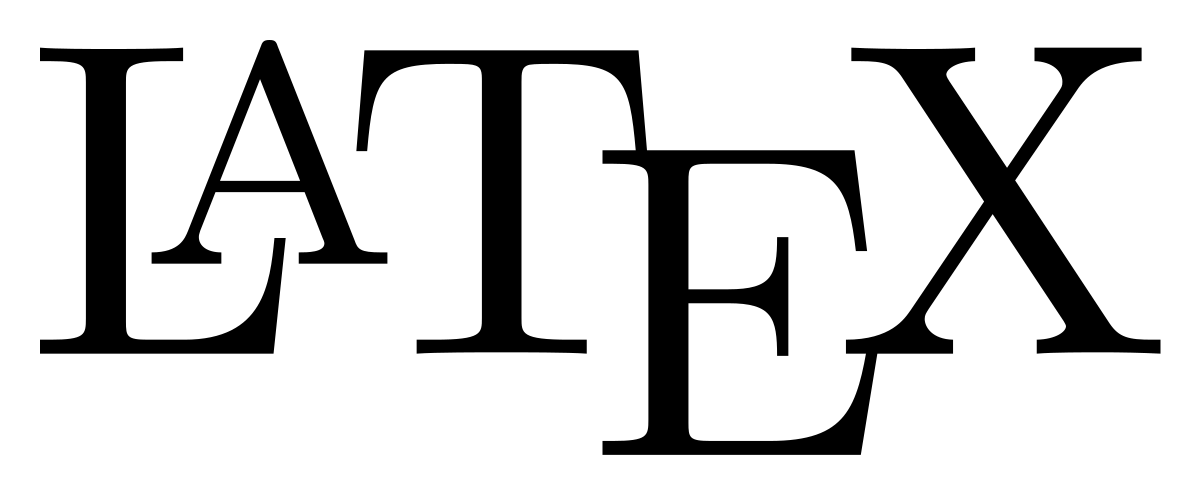
\includegraphics[width=0.6\textwidth]{Bild}
	\caption{Dies ist die Bildunterschrift.}\label{Bild}
\end{figure}

Wenn Sie pdf\LaTeX\ verwenden, können Sie Dateien im jpeg-, png-, oder pdf-Format einbinden, wie mit der Abbildung~\ref{Bild} geschehen. \LaTeX\ dagegen erwartet Dateien ausschließlich im eps- oder ps-Format \cite{andyroberts}.

\subsection{Tabellen}

Hier sei auf die einschlägige Literatur verwiesen, zum Beispiel Referenz~\cite{andyroberts} oder Referenz~\cite{hobbits}.

\subsection{Formeln}

Beim Darstellen von Formeln demonstriert \LaTeX\ seine ganze Stärke. Man kann kurze Formeln in den laufenden Text einbinden, zum Beispiel $a^2+b^2=c^2$, den Satz des Pythagoras. Möchte man abgesetzte Formeln verwenden, die durchnummeriert und referenzierbar sind, verwendet man eine der von \texttt{amsmath} \cite[Table 3.1]{amsmath} bereitgestellten Umgebungen.

\begin{equation}
	\textrm{Student} = \int_\textrm{früh}^\textrm{spät} \mu \; \mathrm{d}e. \label{formel1}
\end{equation}

Auf Formel~(\ref{formel1}), die der geneigte Leser bitte nicht allzu ernst nehmen möge, kann man später verweisen.

\section{Diskussion}

Mit Hilfe der zahlreichen Anleitungen, die online zu finden sind, sind Sie sicher bald in der Lage, Ihr Dokument ganz nach Ihren Wünschen zu erweitern und anzupassen. Früher oder später werden Sie auch auf die vielfältigen Möglichkeiten stoßen, das Layout anzupassen. Hierzu möchte ich Ihnen den einleitenden Text zu dem entsprechenden Kapitel aus Referenz~\cite{lshort} mitgeben:

\begin{quote}
	Chapter 6 contains some potentially dangerous information about how to alter the standard document layout produced by \LaTeX. It will tell you how to change things such that the beautiful output of \LaTeX\ turns ugly or stunning, depending on your abilities.
\end{quote}

\begin{thebibliography}{9}

\bibitem{anleitung}
Anke B.~Schmidt, \emph{Anleitungen zu den Experimentellen Übungen zur \ldots}.

\bibitem{andyroberts}
Andrew Roberts. \emph{Getting to Grips with} \LaTeX, a most useful website: \url{http://www.andy-roberts.net/writing/latex}.

\bibitem{hobbits}
Manuela Jürgens und Thomas Feuerstack, \LaTeX\ \emph{-- eine Einführung und ein bisschen mehr \ldots}, FernUniversität in Hagen, Februar 2013.

\bibitem{amsmath}
User’s Guide for the amsmath Package (Version 2.0): \url{http://mirrors.ctan.org/macros/latex/required/amslatex/math/amsldoc.pdf}.

\bibitem{lshort}
Tobias Oetiker, Hubert Partl, Irene Hyna und Elisabeth Schlegl, \emph{The Not So Short Introduction to} \LaTeX\ 2$\varepsilon$.

\end{thebibliography}

\end{document}
